\documentclass[a4paper]{jctart10}
%\JCTvolume(**,\ *,2015)
%\oddsidemargin=-1.mm \evensidemargin=-4.5mm
\oddsidemargin=-1.5mm \evensidemargin=-2.5mm

\usepackage{amssymb,amsmath}
\usepackage[pdftex]{graphicx}  % Графика для рис.~в pdf и png компил.~--- PDF/LaTeX
\usepackage{epstopdf}
\usepackage{multirow}
\usepackage{hyperref}
%\usepackage{graphicx} % Графика для рис.~в ps (eps) компиляц.~--- LaTeX, затем dvi/pdf


\begin{document}

\setcounter{page}{1}

\markboth{С.\,В.~Панин, В.\,В.~Титков, П.\,С.~Любутин}{Автоматический выбор размера площадки корреляции в задаче оценки ...}


\title{Автоматический выбор размера ядра корреляции\\в задаче оценки деформации материалов\\методом корреляции цифровых изображений\footnote{Работа выполнена в рамках проектов фундаментальных исследований РАН, гранта РФФИ №~13-07-00009 ``Развитие быстродействующих и помехоустойчивых алгоритмов обработки и анализа оптических и акустических сигналов для комбинированного метода контроля состояния нагруженных материалов''.}}

\author{\sc{С.\,В.~Панин$^{1,2}$, В.\,В.~Титков$^1$, П.\,С.~Любутин$^{1,2}$}\\
             $^1${\it Институт физики прочности и материаловедения СО РАН, Томск, Россия}\\
             $^2${\it Национальный исследовательский Томский политехнический университет, Россия}\\
             e-mail: \tt{svp@ispms.tsc.ru}}

    \date{}
     \maketitle

\begin{abstract}
Предложен алгоритм выбора размера ядра корреляции при построении полей векторов перемещений методом корреляции цифровых изображений. Проведено тестирование алгоритма на модельных и экспериментально полученных оптических изображениях, характеризуемых различной текстурой. Исследовано влияние размера ядра корреляции и текстуры изображения на помехоустойчивость определения перемещений. Показано, что предлагаемый алгоритм позволяет определить размер ядра корреляции, обеспечивающий минимальную ошибку определения перемещений и оценки деформации.

{\it Ключевые слова}: размер площадки корреляции, векторное поле, интенсивность деформации сдвига, корреляция цифровых изображений.
\end{abstract}

\section*{Введение}

Оптический метод оценки деформации, основанный на корреляции цифровых изображений (именуемый в зарубежной литературе {DIC}~--- digital image correlation), включает два основных этапа: 1) построение поля векторов перемещений и 2) последующий расчет компонент деформации~\cite{1}. Большинство исследований в области разработки алгоритмов построения векторов перемещений направлены на повышение точности и увеличение помехоустойчивости определения смещений~\cite{2, 3}, либо увеличение быстродействия.

В современных DIC-системах перед нагружением на поверхности исследуемого материала с помощью двух баллонов краски формируется спекл-картина~\cite{1}. Это позволяет повысить контрастность и обеспечить достоверное определение перемещений. При этом форма и размер элементов спекла могут существенно влиять на точность и помехоустойчивость измерения смещений. В работе~\cite{4} исследовано влияние размера элементов спекла (пятен) на точность определения смещений методом DIC. Погрешность измерения определялась как сумма систематической ошибки, вызванной субпиксельной ошибкой при определении смещений, и случайной погрешности, обусловленной наличием шумов и их уровнем. Показано, что радиус пятен в спекле порядка 3~$\sim$~4 пикселов обеспечивает минимальную ошибку определения смещения.

Помимо выявления оптимального размера элементов спекла, существует проблема выбора размера ядра корреляции. Под ядром корреляции подразумевается площадка изображения, для которой определяется перемещение, и её центр соответствует координатам искомого вектора перемещений. В зарубежной литературе для обозначения размеров фрагментов изображений, участвующих в работе корреляционного алгоритма, применятся термин subset size. Далее в статье будем использовать термин «размер площадки корреляции», который по нашему мнению наиболее соответствует термину subset size. Заметим, что в методе определения оптического потока площадка корреляции, как правило, соответствует небольшим по площади фрагментам изображения, что обусловлено, прежде всего, необходимостью снижения вычислительных затрат при построении полного поля перемещений, а также обеспечения достаточно высокой плотности векторов поля перемещений~\cite{5, 6, 7}. Наличие шумов на изображении, деформация наблюдаемых объектов, а также малый размер площадки корреляции обуславливают появление ошибок в оценке перемещений. Частично, проблема их наличия может быть решена пост-корректировкой поля векторов перемещений, в качестве которой используются пространственная фильтрация~\cite{8}, сглаживание~\cite{9} и т. п. Другим способом решения проблемы влияния шумов является увеличение размера площадки корреляции~\cite{10, 11}. Увеличение размера площадки корреляции приводит к усреднению величин перемещений. Такое усреднение в большинстве случаев также негативно сказывается на точности определения деформации, в том числе, когда перемещения соседних участков отличаются друг от друга по величине и направлению. Таким образом, размер площадки корреляции должен иметь достаточный размер для сопоставления участков изображений и минимизации влияния помех и шумов и с другой стороны приводить к минимальному сглаживанию поля векторов перемещений.

В работе~\cite{12} исследовали проблему выбора размера площадки корреляции и в качестве варианта ее решения предложен подход, в основе которого лежит определение суммы квадратов градиентов интенсивности участков изображения {SSSIG} (Sum of Square of Subset Intensity Gradients). Оценено влияние размера площадки корреляции, а также шума на изображении на ошибку определения перемещений. В~\cite{1} приводятся рекомендации для выбора размера площадки корреляции в зависимости от физического размера образца материала, изображенного на фотографии, а также от разрешения изображения (оптической системы) и размера элементов спекла (пятен). Приведенная информация является скорее рекомендацией по проведению съемки материалов для обеспечения требуемой точности, чем конкретным алгоритмом выбора размера площадки корреляции.

Таким образом, проблема автоматического выбора размера площадки корреляции (subset size), содержащей достаточно уникальные и идентифицируемые особенности (объекты на изображении) для обеспечения надежного и точного определения смещений, является предметом исследований. В настоящей работе была поставлена задача разработки алгоритма выбора размера площадки корреляции без использования дополнительной информации об условиях съемки (распределении шума на изображении, размере элементов спекла и т.п.), а также без участия оператора (т.е. без предварительного задания каких-либо параметров расчета).

\section{Алгоритм выбора размера площадки корреляции}
\begin{figure}[b!]
    \centering
		\small{\it а}\\
    \includegraphics[width=80mm]{ris/1a.png}\\
		%\caption{а}
		{\it б}\\
		\includegraphics[width=170mm]{ris/1b.png}
		%\caption{б}
    \caption{К пояснению определения смещений. ({\it а}) принцип построения поля векторов перемещений; ({\it б}) пример распределения автокорреляционной функции для трех значений {\it n}:
1 – {\it n} = 8, 2 – {\it n} = 64, 3 – {\it n} = 512.}
\end{figure}

Как было указано выше, один из основных этапов метода {DIC} -- это построение поля векторов перемещений. Алгоритм определения перемещений основан на установлении соответствия между участками двух изображений путем вычисления взаимнокорреляционной функции (ВКФ) и поиске ее экстремума~\cite{13}. Нахождение максимума ВКФ в пределах зоны сканирования производится построчно с шагом 1 пиксел. Размер зоны сканирования ($sa$) и шаг построения векторов ($step$) (рис. 1, {\it а}) изначально задаются оператором. На рис.~1, а приняты следующие обозначения: $n$~--- размер стороны площадки, в пределах которой вычисляется коэффициент корреляции; $sa$~--- размер стороны зоны сканирования; $step$~--- шаг построения векторов; $I_{Э}$, $J_{Э}$~--- координаты левого верхнего угла участка изображения.

В настоящей работе предлагается алгоритм определения размера площадки корреляции $CA$ из набора значений $n$, лежащих в диапазоне $0 < n < min\{w/4;h/4\}$, где $w$~и~$h$~--- ширина и высота изображения, $min$~--- оператор выбора минимального значения аргументов (параметров изображения) (рис.~2). При функционировании алгоритма необходимо учитывать, что увеличение размера $n$ приводит к возрастанию объема вычислений, а также к усреднению оценки перемещений, т. е. потере точности оценки деформации. В то же время уменьшение $n$, в силу недостаточности локальной информации, может вызвать ошибки оценки перемещений. Это связано с тем, что различные участки могут иметь похожий характер распределения яркости. Если на изображении имеются области с примерно равной яркостью пикселов, т.е. области низкой контрастности, то значение коэффициента корреляции для пар таких областей будет стремиться к единице. Это может привести к возникновению ошибок при построении векторного поля, так как найденное смещение может отвечать как искомому участку, так и приводить к построению некорректного вектора. Таким образом, на основании изложенного, был предложен алгоритм, основанный на вычислении автокорреляционной функции и количественной ее характеризации, включающий следующие этапы.
\begin{enumerate}
\item На первом этапе вычисляются значения автокорреляционной функции в горизонтальном и вертикальном направлениях. Для расчета используется нормированный коэффициент корреляции с нулевым средним~\cite{13, 14}.
\begin{equation}
ZNCC =\frac{\sum(X-\overline{X})(Y-\overline{Y})}{\sqrt{\sum(X-\overline{X})^{2}(Y-\overline{Y})^{2}}}
\end{equation}
где $X$, $Y$~--- яркости сравниваемых участков изображения;
$\overline{X} = \frac{1}{n}\sum^{n}_{t=1}X_{t}$,\\*$\overline{Y}~=~\frac{1}{n}\sum^{n}_{t=1}Y_{t}$~--- средние значения яркостей тех же участков. Каждое значение автокорреляционных функций вычисляется как среднеарифметическое для трех строк либо трех столбцов изображения соответственно. Расчеты проводятся для первых, центральных, последних строк и столбцов соответственно (таких, чтобы размеры сравниваемых участков вписывались в изображение). Для строки/столбца автокорреляционная функция вычисляется относительно центрального участка размером $n \times n$ пикселов с шагом в один пиксел.
\item Для рассчитанных значений автокорреляционной функции в горизонтальном и вертикальном направлениях для параметра $n$, изменяющегося в диапазоне $2 < n < 64$, вычисляются следующие параметры:

$FS$~--- ширина автокорреляционной функции ($ZNCC$) на уровне 0.5 в пикселях (рис. 1,б);

$N$~--- количество малоконтрастных областей на изображении. Малоконтрастными будем считать области, в которых яркости пикселов имеют среднеквадратическое отклонение меньше заданного порога. В настоящей работе использовался порог равный 10. В таких областях отсутствуют заметные перепады яркости, связанные, например, с наличием трещин на поверхности, границами структурных элементов, нанесенными элементами спекла и т.п. Это приводит к тому, что невозможно найти соответствие между участками изображений, так как в формуле (1) величина разности стремится к нулю;

$P$~--- количество пиков автокорреляционной функции, превышающих уровень 0.5. Данный параметр характеризует количество областей изображения, подобных по распределению яркости.
\item Этапы 1–2 повторяются для различных $n$.
\item Выбирается минимальная величина $n$, для которой выполняются следующие условия, с целью выбора размера $CA$:
\begin{itemize}
	\item количество пиков $P$ должно равняться 1, то есть каждый участок изображения размером $n \times n$ должен иметь достаточно уникальное распределение яркости;
	\item количество областей $N$ на изображении, для которых выполняется условие низкой контрастности (см. выше этап~2) должно быть равным нулю, то есть все области изображения должны характеризоваться значительными перепадами яркости.
\end{itemize}
\item Затем, начиная с выбранного на 4-ом этапе значения $n$, подбирается такое, для которого величина параметра $FS$ будет меньше или равно, такового, рассчитанного при следующем значении $n$ (рис.~2). Полученное значение и принимается в качестве искомого $CA$.
\end{enumerate}
\begin{figure}[b!]
    \centering
    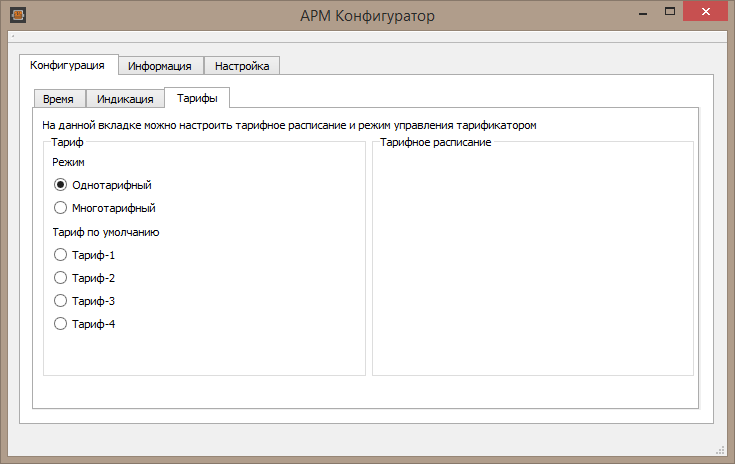
\includegraphics[width=100mm]{ris/2.eps}\\
    \caption{Схема алгоритма выбора размера площадки корреляции ($n_{i}$~--- значение $n$ на $i$-ой итерации алгоритма).}
\end{figure}
Если в процессе работы алгоритма какое-либо из условий не выполняется, это будет свидетельствовать о недостаточно контрастной текстуре изображения. Если эту проблему невозможно решить путем формирования на поверхности объекта измерения достаточно контрастной спекл-картины, то следует принять тот размер $CA$, которому соответствуют минимальные значения параметров $P$ и $N$.

\section{Методика тестирования}

\subsection{Формирование серий тестовых изображений}

В общей постановке генерация серий модельных изображений состоит из двух этапов: 1) формирование изображения модельной поверхности; 2) формирование серии изображений модельной поверхности с учетом приращения деформации. Всего исследовали 6 серий изображений, три из которых были модельными (полученными искусственно).

\begin{figure}[htbp]
    \centering
		\small{\it а) серия 1}\hspace*{75mm}{\it б) серия 2}\\[2mm]
    \includegraphics[width=60mm]{ris/3a.png}\hspace*{15mm}
		%\caption{а) серия 1}
		\includegraphics[width=60mm]{ris/3b.png}\\
		%\caption{б) серия 2}
		{\it в) серия 3}\hspace*{75mm}{\it г) серия 4}\\[2mm]
		\includegraphics[width=60mm]{ris/3c.png}\hspace*{15mm}
		%\caption{в) серия 3}
		\includegraphics[width=60mm]{ris/3d.png}\\
		%\caption{г) серия 4}
		{\it д) серия 5}\hspace*{75mm}{\it е) серия 6}\\[2mm]
		\includegraphics[width=60mm]{ris/3e.png}\hspace*{15mm}
		%\caption{д) серия 5}
		\includegraphics[width=60mm]{ris/3f.png}
		%\caption{е) серия 6}
    \caption{Примеры модельных и экспериментальных изображений.}
\end{figure}

\begin{itemize}
	\item {\it Модель многослойного изображения.} Модельное изображение (рис. 3,\,{\it а}) получали из заданного количества слоев псевдослучайных чисел; при этом каждый слой соответствует определенной пространственной частоте~\cite{15}. Первый слой некоторого заданного исходного размера заполняется псевдослучайными значениями с равномерным распределением. Затем размер данного слоя увеличивается в два раза с помощью интерполирования бикубическим В-сплайном. Второй слой формируется аналогично первому, но перед увеличением его размера он складывается попиксельно с первым. Итеративно генерируются несколько слоев, и на каждой итерации конечный размер изображения увеличивается в два раза. После генерации всех слоев, проводится масштабирование и нормировка яркости в диапазоне от 0 до 255. Таким образом, имея начальный слой размером $4 \times 4$ пиксела, после проведения 8 итераций, получаем модельное изображение размером $1024 \times 1024$ пикселов.
	\item {\it Модель спекла (окрашенной поверхности).} При создании модельного изображения спекла (рис. 3,\,{\it б}) (вторая серия) стояла задача создания изображения подобного экспериментально получаемым при фотографировании образца (рис. 3,\,{\it г}). Для этого изображение «заливали» цветом, подобным по тону оттенку поверхности образца на экспериментально регистрируемых фотографиях. Затем в «случайно» заданных (по нормальному закону распределения) участках генерировали окружности (имитирующие капли распыляемой краски – пятна спекла), радиусом (0 до 10 пикселов), уровень (градация) серого которых задавался случайным образом.
	\item Для третьей модельной серии размер пятен был увеличен в четыре раза (рис. 3,\,{\it в}).	
\end{itemize}
Последующие три серии (4~--~6) были сформированы из экспериментально полученных изображений нагруженных материалов:
\begin{itemize}
	\item {\it Алюминиевый сплав А2024 с напыленным спеклом.} Экспериментально полученное оптическое изображение (рис. 3,\,{\it г}) было записано при растяжении образца алюминиевого сплава А2024, на поверхности которого с помощью аэрозольных баллонов с черной и серой краской была сформирована спекл-картина.
	\item {\it Углерод-углеродный композит с напыленным спеклом.} Данный материал представляет собой псевдоизотропный композит из слоев однонаправленных углеродных лент спеченный в углеродной матрице. Процесс получения изображений поверхности описан в~\cite{16}, пример фотографии изображен на рис. 3,\,{\it д}.
	\item {\it Алюминиевый сплав Д16АТ без напыленного спекла.} На рис. 3,\,{\it е} приведено экспериментально полученное изображение образца алюминиевого сплава Д16АТ, зарегистрированный при проведении механических испытаний на растяжение~\cite{17}.
\end{itemize}
{\it Формирование серии изображений модельной поверхности с учетом приращения деформации.} С целью моделирования изменений поверхности, происходящих при нагружении по схеме одноосного растяжения, задавали смещение каждой точки модельной поверхности. При этом яркость каждого пиксела изображения пересчитывается для заданного приращения деформации. В результате из начального изображения получали серию с заданным конечным приращением деформации и известным распределением векторов перемещений. Таким образом, из начального изображения формируется вся серия, состоящая из заданного количества кадров и отражающая схему одноосного растяжения.

В результате было сгенерировано шесть серий изображений, каждая из которых содержит 6 кадров, имитирующих растяжение образца с приращением деформации 1\% при конечном удлинении 5\%. Далее в тексте серии изображений для краткости будем называть их ``{\it серия 1}'', ``{\it серия 2}'' и т. д.

\subsection{Оценка ошибки определения деформации}

Так как в статье выбрана схема одноосного растяжения, для получения количественной оценки «точности» оценки деформации достаточно оценить ошибку расчета продольной компоненты тензора дисторсии $\varepsilon_{xx}$. Кроме того, поскольку растяжение было равномерное, то заданная и экспериментально рассчитанная величины $\varepsilon_{xx}$ должны быть константами по всему полю. Поэтому ошибку оценивали через среднеарифметическую поэлементную абсолютную разность полей деформации, заданной (модельной) и расчетной $\varepsilon_{xx}$:
\begin{equation}
\delta\varepsilon_{xx} = \frac{1}{N}\sum^{N}_{i=0}|\varepsilon_{xx_{мод_{i}}}-\varepsilon_{xx_{расч_{i}}}|
\end{equation}

\section{Результаты расчетов и их обсуждение}

На рис.~4,\,{\it а} показаны графики изменения анализируемых параметров: $FS$, $N$, $P$ (см.~раздел~2) для модели многослойного изображения (рис. 3,\,{\it а}). Видно, что при малых значениях $n$ указанные параметры характеризуются максимальными значениями (от~30~до~1000), после чего их значения снижаются и остаются на примерно постоянном низком уровне.
\begin{figure}[htbp]
    \centering
		\small{\it а}\\
    \includegraphics[width=170mm]{ris/4a.png}\\
		%\caption{а)}
		{\it б}\hspace*{75mm}{\it в}\\[2mm]
		\includegraphics[width=60mm]{ris/4b.png}\hspace*{15mm}
		%\caption{б)}	
		\includegraphics[width=60mm]{ris/4c.png}\\
		%\caption{в)}
		{\it г}\hspace*{75mm}{\it д}\\[2mm]
		\includegraphics[width=60mm]{ris/4d.png}\hspace*{15mm}
		%\caption{г)}
		\includegraphics[width=60mm]{ris/4e.png}\\
		%\caption{д)}
		{\it е}\hspace*{75mm}{\it ж}\\[2mm]
		\includegraphics[width=60mm]{ris/4f.png}\hspace*{15mm}
		%\caption{е)}
		\includegraphics[width=60mm]{ris/4g.png}
		%\caption{ж)}
    \caption{Зависимости параметров $FS$, $N$, $P$ от размера площадки корреляции {\it n}: {\it а}, {\it б}) серия 1; {\it в}) серия 2; {\it г}) серия 3; {\it д}) серия 4; {\it е}) серия 5; {\it ж}) серия 6.}
\end{figure}

В силу того, что $FS$, $N$, $P$ отличаются по абсолютной величине, для более наглядного отображения была проведена их нормировка до диапазона от~0~до~1 (см.~рис.~4,\,{\it б-ж}). Нормировка представляет собой преобразование вида:
\begin{equation}
x_{норм} = \frac{x-x_{min}}{x_{max}-x_{min}}
\end{equation}
где $x_{min}$~--- минимальное, $x_{max}$~--- максимальное значение величины.
Максимальные значения $FS$, $N$, $P$ при малых величинах $n$ объясняются малым количеством контрастных объектов (неоднородностей) на изображении, которые лежат в пределах площадки корреляции. Из этого следует:
\begin{itemize}
	\item количество пар участков на изображениях с коэффициентом корреляции близким к единице будет достаточно велико (для параметра $P$);
	\item число малоконтрастных областей будет также велико (для параметра $N$);
	\item на распределении автокорреляционной функции будет присутствовать множество пиков с амплитудой больше 0.5, что приведет к высокому итоговому значению параметра $FS$.
\end{itemize}

Последующий спад параметров $FS$, $N$, $P$ по мере увеличения $n$ является следствием возрастания числа лежащих в пределах площадки корреляции объектов (неоднородностей) изображения (например, пятен спекла). Соответственно, число пар участков, имеющих коэффициент корреляции близкий к 1 (параметр~$P$), стремится к единице. Количество малоконтрастных областей будет стремиться к нулю (параметр~$N$); количество пиков на распределении автокорреляционной функции стремится к единице, в то время как ширина пика должна иметь минимальное значение (параметр~$FS$ ). На рис. 4 наблюдается различная крутизна спада характеристик $FS$, $N$, $P$: для серий 1, 3, 6 наблюдается пологий спад; для серий 2, 4, 5 более резкий. Это объясняется степенью контрастности изображений и числом объектов (неоднородностей) на изображении (например, размером пятен спекла, рельефом на поверхности материала и пр.).

Для изображений с достаточно малой контрастностью текстуры (серии 1,~6), а также и для изображений, содержащих относительно крупные малоконтрастные области (объекты) (серия~3) необходимо большее значение $n$ для того, чтобы $FS$, $N$, $P$ достигли минимальных значений. По этой причине характер изменения параметров $FS$, $N$, $P$ по мере возрастания $n$ является более плавным. И, наоборот, для более контрастных изображений (серии~4,~5) и изображений с малым размером пятен спекла (серия~2) уже при относительно небольших значениях $n$ параметры $FS$, $N$, $P$ достигают минимума. В результате наблюдается достаточно резкий спад графиков $FS$, $N$, $P$. В частности, параметр СА возрастает с 10 до 48 (табл.~1) при увеличении в 4 раза размера пятен спекла в модели окрашенной поверхности (серии~2~и~3), что связано с повышением площади малоконтрастных областей (пятен спекла). Для серии 6, так же как и для серии 3, характерна большая величина $СА$ и плавное снижение числа малоконтрастных областей (рис.~4,\,{\it г},~{\it ж}), что ожидаемо, так как поверхность образца серии 6 не окрашена. В то же время для образца с нанесенным спеклом (серия~4), модели окрашенной поверхности (серия~2) и изображений с контрастной поверхностью (серии~1~и~5) наблюдает резкий спад рассчитываемых параметров, что свидетельствует о более помехоустойчивом определении размера $СА$. Таким образом, прослеживается четкая связь между степенью контрастности изображений, характером текстуры на поверхности материала и изменением параметров $FS$, $N$, $P$ по мере увеличения $n$.

Анализ полученных графиков (рис.~4) позволяет выбрать оптимальный размер параметра $n$ (табл.~1) в соответствии с предлагаемым алгоритмом (см.~раздел~1). Для подтверждения оптимальности выбора размера $CA$ были произведены расчеты зависимости ошибки (см.~раздел~2.1) измерения деформации от величины $n$, на основании, которых были определены размеры площадки корреляции при наименьшей ошибке измерения деформации (табл.~1). На рис.~5 приведена зависимость только для серии~4, так как остальные зависимости имеют подобный характер и отличаются только по абсолютным величинам. На рис. 5 видно, что малым значениям $n$ соответствуют большие значения ошибки. С увеличением $n$ последняя уменьшается до некоторого значения ($2 \cdot 10^{-3}$) и при последующем увеличении $n$ остается примерно постоянной. Это объясняется малой контрастностью изображения в пределах площадки корреляции при малых ее размерах. Дальнейшее увеличение $n$ не сопровождается уменьшением ошибки, поскольку количество объектов (неоднородностей) на изображении, приходящихся на единицу площади, далее не возрастает.

Также было замечено, что результаты выбора размера $СА$ не зависят от величины деформации (в рамках проведенных экспериментов и используемых в них диапазона ее изменения), что подтверждается данными графиков на рис.~5. Видно, что для различных экспериментов по растяжению образцов ошибка измерения деформации достигает минимального значения при одном и том же значении $n$.

Из таблицы~1 видно, что определенные в результате работы алгоритма размеры площадки корреляции совпадают со значениями, соответствующими минимальной ошибке $\varepsilon_{xx}$, или незначительно их превышают. При этом если размер площадки больше значения, соответствующего минимальной ошибке $\varepsilon_{xx}$, удается получить даже меньшую ошибку определения деформации по сравнению с использованием меньшего размера площадки. Это связано с тем, что уменьшение размеров $СА$ приводит к появлению большего количества ложных пиков на автокорреляционной функции (см.~график автокорреляционной функции на рис.~1,\,{\it б}).


\begin{center}
\begin{table}[h]
\caption{Результаты расчета параметров при выборе размера \it{СА}}
\begin{tabular}{|c|c|c|c|c|c|}
\hline
\multirow{3}{2.5cm}{Модель изображения} & \multicolumn{5}{c|}{Размер \it{СА}}  \\
\cline{2-6}
& \multicolumn{4}{c|}{По алгоритму, по параметру}  & \multirow{2}{3.3cm}{По~минимальной ошибке~$\varepsilon_{xx}$} \\ \cline{2-5}
& {~~~~~~}$P${~~~~~~} & {~~~~~~}$N${~~~~~~} & {~~~~~~}$FS${~~~~~~} & {~~~}Итог{~~~} &    \\
\hline
1   & 16             & 16             & 16              & 16   & 14    \\
\hline
2    & 10             & 10             & 10              & 10   & 10  \\
\hline
3                                   & 26             & 48             & 48              & 48   & 46                                     \\ \hline
4                                   & 14             & 12             & 16              & 16   & 12                                     \\ \hline
5                                   & 12             & 12             & 12              & 12   & 10                                     \\ \hline
6                                   & 22             & 52             & 52              & 52   & 42                                     \\ \hline
\end{tabular}
\end{table}
\end{center}

\begin{figure}[htbp]
    \centering
    \includegraphics[width=60mm]{ris/5.png}
    \caption{Зависимости средней ошибки расчета деформации $\varepsilon_{xx}$ от параметра $n$ в зависимости от степени деформации: 1) 1\%, 2) 3\%, 3) 5\%.}
\end{figure}

Из проведенного исследования видно, что алгоритм позволяет успешно проводить обработку, как модельных, так и экспериментальных изображений. Модельному изображению (серия~3) и экспериментальному (серия~6) с малой контрастностью, соответствуют более пологие графики зависимостей параметров $FS$, $N$, $P$ от $CA$. Остальные серии изображений как модельные, так и экспериментальные, с более контрастной текстурой, имеют более круто меняющиеся зависимости. Таким образом, на основании полученных данных (рис.~4,~5, и табл.~1) и их анализа можно сделать вывод, что предлагаемый алгоритм может быть эффективно использован на практике.

Помимо основных выводов, связанных с работой алгоритма, из проведенных исследований можно заключить, что характер текстуры поверхности (включая размер пятен спекла) и степень контрастности изображения оказывают существенное влияние на подбор оптимальных параметров алгоритмов построения векторного поля, а значит и на точность и достоверность измерения деформации материалов методом корреляции цифровых изображений. В частности, очевидна прямая зависимость между размером пятен спекла и размером площадки корреляции: при радиусе пятен 0-10 пикселов в серии 2~--- оптимальны размер $CA$ равен 10, а при радиусе 0-40 пикселов в серии 3~--- $СА$ равен 48 (причем, из проведенных авторами расчетов, не вошедших в статью, для серий с большим радиусом пятен спекла данная линейная зависимость сохранялась). Стоит отметить, что полученные ниспадающие зависимости ошибки расчета деформации от размера площадки корреляции согласуются с исследованиями, изложенными в~\cite{12}, как по характеру изменения кривой, так и по большим абсолютным ошибкам для менее контрастных изображений.

\section*{Заключение}

В работе предложен алгоритм автоматического выбора размера площадки корреляции в задаче построения векторных полей при оценке деформации методом корреляции цифровых изображений. Проведены исследования работы алгоритма на модельных и экспериментальных данных. По результатам выполнения алгоритма для шести серий изображений с различным характером текстуры определены размеры площадки корреляции, обеспечивающие минимальную ошибку оценки деформации.

Проведено сравнение выявленных в результате применения алгоритма размеров с величинами размера площадки корреляции, при которых ошибка определения деформации достигает минимального значения. Найдены значения размера площадки корреляции, которым соответствует минимум ошибки. При сравнении значений, определенных с помощью алгоритма, и значений, соответствующих минимальной ошибке, установлено незначительное отклонение первых в большую сторону. Таким образом, разработанный алгоритм эффективен при измерении деформации материалов, имеющих различный рельеф, включая обработку изображений подготовленных (с напыленным спеклом) так и неподготовленных (малоконтрастных) поверхностей.

\begin{thebibliography}{99}

		 \bibitem{1} {\sc Sutton M. A., Orteu J.-J., Schreier H.} Image correlation for shape, motion and deformation measurements: basic concepts, theory and applications. Springer. 2009, 321~p.
		
			\bibitem{2} {\sc L. Xu, J. Jia, and Y. Matsushita.} Motion detail preserving optical flow estimation. // PAMI 34(9):1744-1757, 2012

		  \bibitem{3} {\sc Sun, D., Sudderth, E. and Black, M.J.} Layered segmentation and optical flow estimation over time. Computer Vision and Pattern Recognition (CVPR), IEEE, pages~1768-1775, 2012.
		
			\bibitem{4} {\sc Wang Z.,Li Li’an,Wang S.} Optimization of Speckle Size in Digital Image Correlation Method[OL]. [ 5 February 2010] \url{http://www.paper.edu.cn/en_releasepaper/content/39956}.
		
			 \bibitem{5} {\sc B.K.P. Horn and B.G. Schunck.} Determining optical flow, Artificial Intelligence, Vol. 17, 1981, pp.~185-203.
		
		 \bibitem{6} {\sc B. D. Lucas and T. Kanade.} An iterative image registration technique with an application to stereo vision // Proceedings of Image Understanding Workshop, 1981, pp.~121-130.
		
		 \bibitem{7} {\sc P. Anandan. } A computational framework and an algorithm for the measurement of visual motion, International Journal of Computer Vision, Vol.~2, 1989, pp.~283-310.
		
		 \bibitem{8} {\sc Панин~С.В., Титков~В.В., Любутин~П.С.} Исследование эффективности алгоритмов фильтрации векторных полей при оценке деформации материалов методом корреляции цифровых изображений // Автометрия, 2013, Т.~49, №2, с.~57-67.
		
		 \bibitem{9} {\sc Панин~С.В., Титков~В.В., Любутин~П.С.} Сглаживание векторных полей с использованием поверхности Безье при оценке деформации методом корреляции цифровых изображений // Автометрия, 2014, Т.~50, №1, С.~74-81.
		
		 \bibitem{10} {\sc Hanna, K.} Direct multi-resolution estimation of ego-motion and structure from motion. In IEEE Workshop on Visual Motion, Princeton, NJ, 1991, pp.~156–162.
		
		 \bibitem{11} {\sc Stein, G.P. and Shashua A.} 1997. Model-based brightness constraints: On direct estimation of structure and motion. In IEEE Conference on Computer Vision and Pattern Recognition, San-Juan, pp.~400-406.
		
		 \bibitem{12} {\sc Pan B, Xie H, Wang Z, Qian K, Wang Z.} Study on subset size selection in digital image correlation for speckle patterns. Opt Express. 2008;16(10):7037-7048.
		
		 \bibitem{13} {\sc Панин С.В., Сырямкин В.И., Любутин П.С.} Оценка деформации твердых тел по изображениям поверхности // Автометрия. 2005. Т. ~41, №2. С.~44-58.
		
		 \bibitem{14} {\sc Giachetti A.} Matching techniques to compute image motion // Image and Vision Computting. 2000. Vol.~18. P.~247-260.
		
		 \bibitem{15} {\sc Панин С.В., Титков В.В., Любутин П.С.} Инкрементный подход к определению перемещений фрагментов изображений при построении векторных полей. Автометрия, 2014, Т.~50, №2. С.~39-49.
				
		 \bibitem{16} {\sc Панин С.В., Бурков М.В., Бяков А.В. и др.} Стадийность деформации и разрушения при испытании на срез образцов углерод-углеродного композиционного материала по данным акустической эмиссии, корреляции цифровых изображений и тензометрии // Известия ВУЗов. Физика – 2012 – Т.~55 – №5/2 – C.~228-233.
		
		 \bibitem{17} {\sc Панин С.В., Бяков А.В., Гренке В.В., Шакиров И.В., Юссиф С.А.К.} Многомасштабное исследование стадийности локализованной пластической деформации при растяжении образцов сплава Д16АТ с надрезами акустико-эмиссионным и оптико-телевизионным методами // Физ. мезомех. 2009. Т.~12. №6. С.~63-72.

		
\end{thebibliography}

%\vspace*{7mm} {\footnotesize\it \hfill  Поступила в редакцию ** декабря 2014 г.

%\hfill с доработки~--- ** ***** 2015 г.}

\end{document}
